
\chapter{User manual}

This document constitutes the user manual for Psychosynth, it is
intended to help resolve issues in the use of the Psychosynth software
package.\footnote{This document was first written in Spanish,
  available here:

  \url{http://psychosynth.com/index.php/User_manual/es}. 

  This document is a modified version of Ben Mullet's translation of
  that document, which is also accessible in the software's web page,
  integrating other older documents like the ``Installation Guide''.

\url{http://psychosynth.com/index.php/User_manual}}

\section{Installation}

\subsection{Installing from the source code}

First of all you must get a copy of the sources of this program. Go to
the \emph{download
  section}\footnote{\url{http://psychosynth.com/index.php/Download}}
if you do not have them yet. Note that this section describes only how
to install from the source code --- if there is a binary package for
your distribution, use that instead.

\subsubsection{Dependencies}

Then, to try the software you will need these third party libraries
and programs:

\begin{itemize}
\item GNU Autotools (only for the development version) 
\item Ogre (needed by
  the 3D interface)
\item CEGUI (needed by the 3D interface)
\item OIS (needed by the 3D interface)
\item liblo (needed for the network support)
\item libxml2 (needed for XML config support)
\item Alsa (needed for ALSA sound output)
\item Jack (needed for Jack sound ouput) 
\item libsndfile (needed for
  pcm file support) 
\item libvorbis (needed for OGG vorbis file support)
\item SoundTouch (needed for sample stretching)
\item Several Boost libraries
\end{itemize}

In Debian and Ubuntu you can install all those dependencies with the
following command. Anyways, I suggest installing \emph{liblo} from the
original sources because the version in the repositories is outdated
and contains a bug:

\begin{verbatim}
# apt-get install automake libtool libogre-dev \
      libceguiogre-dev libois-dev libcegui-mk2-dev \
      libasound2-dev libjack-dev liblo0-dev \ 
      libsndfile-dev libxml2-dev libsoundtouch1-dev \
      libvorbis-dev libboost-all-dev
\end{verbatim}

\subsubsection{Installing}

If you downloaded the program from Bazaar you will first need to
generate the compilation scripts:
\begin{verbatim}
$ autoreconf
\end{verbatim}

Now you will need to run the configuration script to detect the the
libraries and set up the compilation settings.
\begin{verbatim}
$ ./configure
\end{verbatim}

Check that everything has been detected correctly and that everything
that you want to install is going to be actually built --- for
example, if you did not install Ogre, the library and CLI interface
will install anyway but you will miss the 3D interface. Then compile
the program:
\begin{verbatim}
$ make
\end{verbatim}
At last we must run these commands with superuser privileges to install:
\begin{verbatim}
$ make install
$ ldconfig
\end{verbatim}
We can now run the 3D simulator and enjoy:
\begin{verbatim}
$ psynth3d
\end{verbatim}

\subsubsection{Troubleshooting}

\begin{troubleshoot}
  On Ubuntu 8.10 or Debian Sid I get a linkage problem related to
  CEGUI::Exception
\end{troubleshoot}

You must add this repository to your
\type{sources.list} and update Ogre and Cegui to their latest
versions:

\begin{verbatim}
deb http://ppa.launchpad.net/andrewfenn/ubuntu hardy main
\end{verbatim}

\begin{troubleshoot}
  On Ubuntu 8.04 I can't find Boost 0.35
\end{troubleshoot}

You can find proper \type{.deb} packages here: 
\url{https://launchpad.net/ubuntu/intrepid/+source/boost1.35/}

\begin{troubleshoot}
  On Ubuntu 8.04 I have properly installed \emph{libsoundtouch} but it
  is not detected
\end{troubleshoot}

Run this command before executing configure:

\begin{verbatim}
$ sed s/soundtouch-1.0/libSoundTouch/ configure > configure
\end{verbatim}

\subsection{Installation for Ubuntu and derivatives}

Follow these instructions to install Psychosynth if you are using
Ubuntu or any other derivative (like Trisquel
GNU/Linux\footnote{\url{http://trisquel.info/}}, a fully free, as in
freedom, distribution).\footnote{Thanks a lot to Aleksander Morgado
  who made these packages and wrote this section.}

These packages have been tested in Ubuntu Lucid (10.04), Ubuntu
Maverick (10.10) and Ubuntu Natty (11.04), as well as other older
releases not covered in this PPA.

Please note that since Maverick, the Ubuntu kernel comes without OSS
support, so only ALSA or JACK output are supported. See the
Troubleshooting section below.

\subsubsection{Easy setup}

If you just want to go the easy way, execute these commands:

\begin{verbatim}
$ sudo apt-add-repository ppa:gnu-psychosynth-team/ppa
$ sudo apt-get update
$ sudo apt-get install psychosynth-gui psychosynth-samples 
\end{verbatim}

\subsubsection{Manual setup}

In case you maintain manually your sources.list, here you have the
detailed manual setup instructions. More information can be found in
the GNU Psychosynth PPA webpage.
\begin{verbatim}
deb https://launchpad.net/~gnu-psychosynth-team/+archive/ppa lucid main
deb-src https://launchpad.net/~gnu-psychosynth-team/+archive/ppa lucid main
\end{verbatim}

Where it says lucid you may also write a later version of the Ubuntu
distribution (e.g Maverick). You may need to tell apt to accept those
repos without issuing a warning when running apt-get update. For that,
you can just do the following for each warned key:
\begin{verbatim}
$ gpg --keyserver subkeys.pgp.net --recv 4A3B72F02ADA7053
$ gpg --export --armor 4A3B72F02ADA7053 | sudo apt-key add - 
\end{verbatim}

Once you run \type{sudo apt-get update}, install the packages:
\begin{verbatim}
$ sudo apt-get update
$ sudo apt-get install psychosynth-gui psychosynth-samples 
\end{verbatim}

\subsubsection{Troubleshooting}

\begin{troubleshoot}
Sound comes terribly delayed (up to 30s).
\end{troubleshoot}

If you have ALSA configured in \emph{Settings $\rightarrow$ Audio
  $\rightarrow$ Output} and you get the audio veeeery delayed, then
try to use another Alsa device instead of the \type{'default'} one, like
\type{'hw:0,0'}:
\begin{verbatim}
$ psynth3d -o alsa --alsa-device hw:0,0
\end{verbatim}

\begin{troubleshoot}
No sound yet!
\end{troubleshoot}

Try to use JACK output, this always fixes the problem, in
\emph{Settings $\rightarrow$ Audio
  $\rightarrow$ Output}:
\begin{verbatim}
$ sudo apt-get install jackd
$ jackd -d alsa &
$ psynth3d -o jack
\end{verbatim}

\section{3D user interface}

Psychosynth comes with different programs that allow you to
graphically manipulate synthesizer elements or communicate among
them. Right now there are two user interfaces, a three-dimensional
graphical interface and the command line.

To run the 3D interface enter the command:
\begin{verbatim}
$ psynth3d
\end{verbatim}

Then you should see a window like in figure \ref{fig:userman-0}.

\begin{figure}[h!]
  \centering
  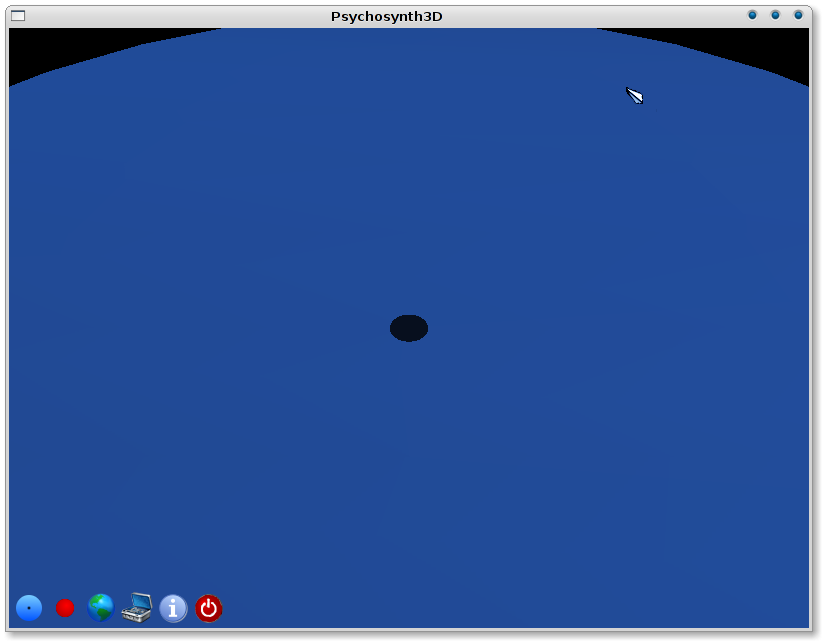
\includegraphics[width=.7\textwidth]{pic/userman-0.png}
  \caption{Initial state of 3D the user interface.}
  \label{fig:userman-0}
\end{figure}

At the bottom of the screen are a series of icon buttons that will
enable us to deploy different windows to control Psychosynth. In the
following order, the buttons are:

\begin{description}
\item[Object Selector] Selects objects to place on the workspace.
\item[Sound Recorder] Records to a file all the sound being generated.
\item[Network Sessions] Connects the synthesizer with others across a
  network.
\item[Info Panel] Displays information panels about the program and
  some help.
\item[Exit] Exit the program.
\end{description}

In the center of the screen is a blue table where Psychosynth objects
are placed to create and manipulate sound, as we shall see below.

Now let's see how we might do this in a three-dimensional environment.

\subsection{The camera}

The first thing we must get used to is manipulating the
\emph{camera}. It might seem that the environment is only 3D eye
candy; in practise it adds important aspects of control over the
synthesiser.

3D provides an intuitive means to adjust a Psychosynth object's
controls: when zoomed out we can see many objects and easily move them
between relatively distant points. On the other hand it is better to
zoom in when we wish to modify an object parameter precisely. Mouse
movements will represent shorter distances and thus increase the
resolution.

Camera movements include:

\begin{description}
\item[Move] To move the camera simply click the left mouse button on
  the table. The whole environment can be dragged around with the
  mouse. We can also focus the camera on a point by pressing the shift
  key while clicking the left button where we want to focus on the
  table.
\item[Rotate] With no object selected we can rotate the camera focus
  around to a given point by moving the mouse while pressing the left
  button
\item[Zoom] We can zoom the point that we have focused by either using
  the mouse wheel or by pressing the middle mouse button while moving
  the mouse forward and backward.
\end{description}

\subsection{Creating sounds}

To create sounds we will be placing some Psychosynth objects on the
table. The central spot represents the main audio output, which will
normally be our speaker.

To \textbf{place an object} on the table, click on the first icon
button at the bottom of the screen. An object selector appears, the
buttons are organized by category - allowing us to select and place
different synthesis objects.

As the library of objects is growing rapidly there is no documentation
yet on individual elements. Fortunately Psychosynth quickly allows you
to experiment with the objects --- discovering what each one does and
how they interact with each other --- learning about audio synthesis
in a fast, fun and highly intuitive manner.

When you click on one of the selector buttons you'll see a yellow
circle that follows the mouse, indicating where the object will be
placed. Then when we click on the table the object will appear
there. If a sinusoidal oscillator is placed it will automatically
connect with the center making a pure tone of 220 Hz.

The situation would then look like in figure \ref{fig:userman-1}

\begin{figure}[h!]
  \centering
  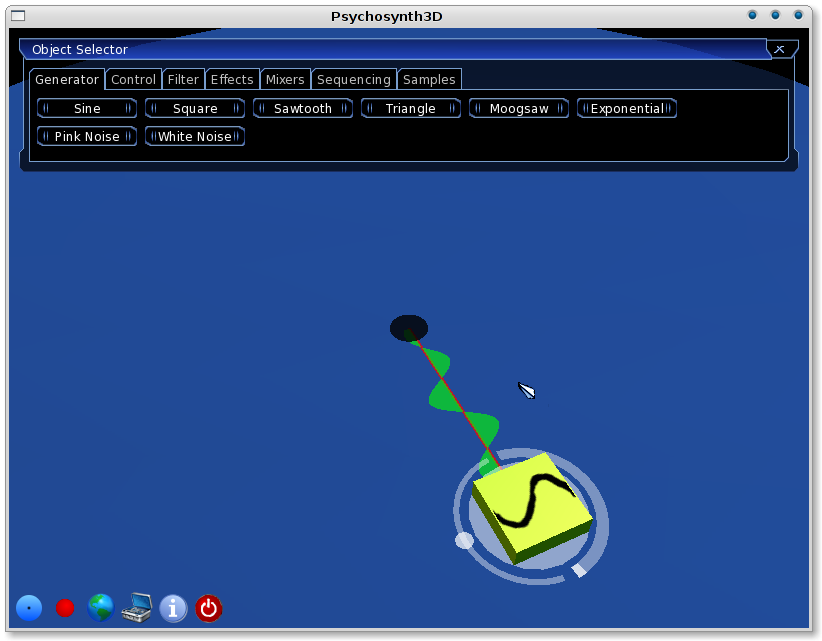
\includegraphics[width=.7\textwidth]{pic/userman-1.png}
  \caption{A simple pure tone generator.}
  \label{fig:userman-1}
\end{figure}

A connection between two objects will show us the wave being broadcast
through it in real time, green if an acoustic signal and yellow if a
control signal.

\subsection{Modifying the sound}

Psychosynth objects are connected with each other automatically. Two
objects will be connected if they have compatible input and output
ports, and if those ports are not already being used for other,
shorter connections. Thus we can very quickly and intuitively alter
the topology of the synthesizer simply by moving the objects that we
want to connect more closely.

To \textbf{move an object}, click the left mouse button and drag it
onto the table.

Each object also has a number of \textbf{parameters}. For example, an
oscillator object like the one we used earlier has two parameters ---
frequency and amplitude (or volume). The frequency is the \textbf{main
parameter} of this object and we can see the relative value on an
indicator that surrounds the subject on the right side.

To modify the main parameter simply move the mouse around the selected
object while holding down the right mouse button, which rotates the
object.

The other parameter --- in this case the amplitude --- is represented
by a slider on the other side of the object. To change it click the
link to the left of the object and move the slider.

There may be other parameters that are not directly represented on the
object, sometimes because they are less important and sometimes
because it is not yet decided how to represent them visually. For
example, the main parameter of a sampler is the playback speed --- the
amplitude is \emph{secondary}. But we can also alter the Tempo
independently --- that is, change the playback speed without changing
the key --- and alter the pitch --- play in a different key without
changing the playback speed.

To list all of an object's parameters and to view and modify the
numerical values, press the \emph{'e'} key to display a parameters
window. An example would be like in figure \ref{fig:userman-2}, this
time showing a more complex scenario.

\begin{figure}[h!]
  \centering
  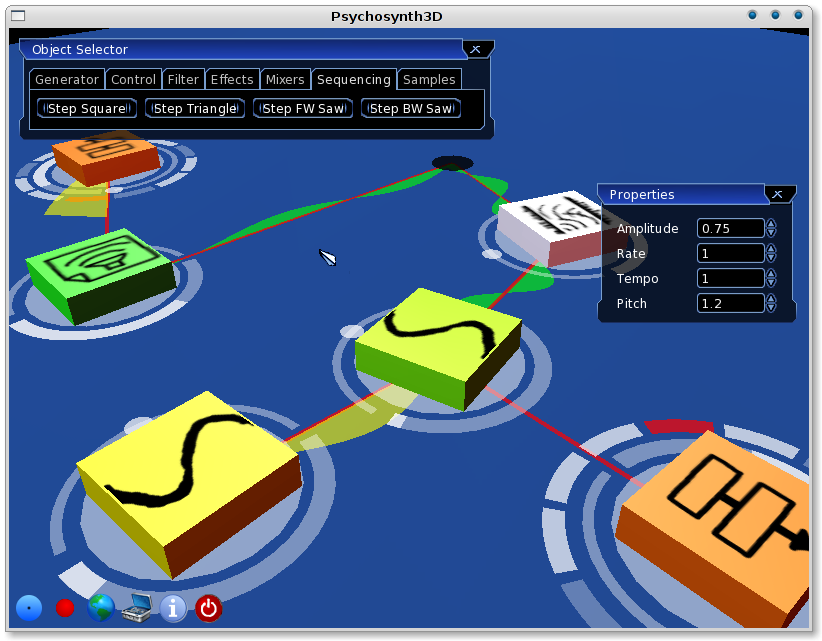
\includegraphics[width=.7\textwidth]{pic/userman-2.png}
  \caption{A complex patch showing the full parameter editor.}
  \label{fig:userman-2}
\end{figure}

To \textbf{remove an object} from the table use the \emph{'delete'} key.

We can also \textbf{select multiple objects} simultaneously which is
useful if modifying their main parameters all at once --- or deleting
them --- or perhaps moving them. To select multiple objects, hold down
the shift key while selecting. To deselect an object in the group
press the control key and click on the object.

Finally, we can temporarily \textbf{mute a connection} by clicking on
it. It then turns black and any objects that attach to that connection
in the hierarchy from the center will not be updated until we click on
that link again.

\subsection{Recording sound}

To \textbf{record a session} just click on the red button that appears
in the second position below. A window appears with the file name to
which the sound is to be saved --- and a start button. Figure
\ref{fig:userman-3} represents this situation.

\begin{figure}[h!]
  \centering
  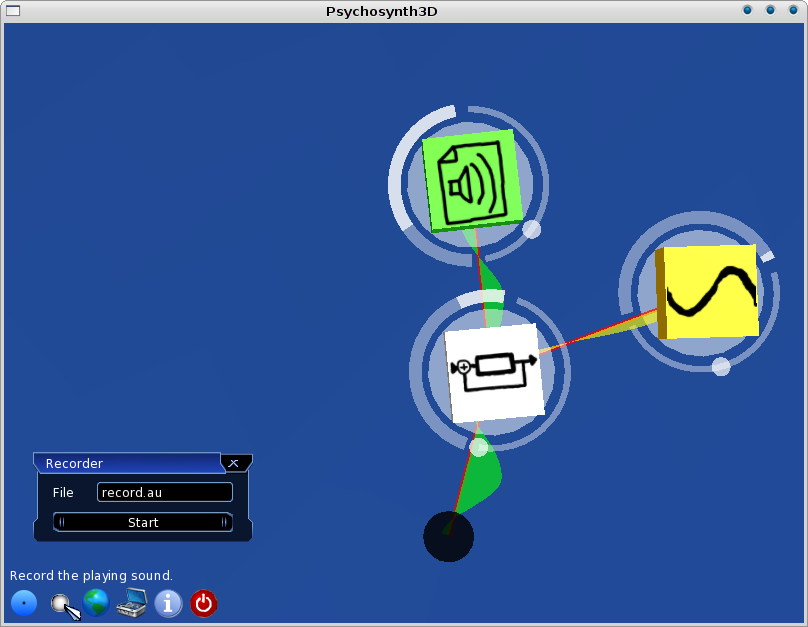
\includegraphics[width=.7\textwidth]{pic/userman-3.png}
  \caption{The session recording dialog.}
  \label{fig:userman-3}
\end{figure}

We can modify the file name to be created, using any valid route from
the current working directory. To start recording, click on Start and
once finished, click on Stop.

\subsection{Network sessions}

To connect multiple synthesisers we need to establish a server
computer and create one or more clients.

During a network session all events will be synchronized between
connected synthesisers, but they will not be aware of any events that
occurred before the connection. Therefore, it is recommended to clear
the table before all computers are connected.

The third icon button in the row below the window opens network
handling, which has two tabs, \emph{client} and \emph{server}. First,
we need a \textbf{server} computer, so we go to the \emph{server}
tab. Then we can alter the listening port number - usually the default
port is used. When you start the server it will be ready to receive
connections and the box in the window displays: \emph{``Server
listening''}. The same box will show when someone is connected or
disconnected --- and similar events.

The other computers use the tab \emph{client} to connect as
\textbf{clients}. There we enter the IP address of the computer server
where it says \emph{Remote host} and the port in \emph{Remote
  port}. We can also change the client listening port in \emph{Local
port}. Once we are ready to go, hit the \emph{start} button.

A message that says \emph{``Connecting...''} should appear. Once the
connection has been made successfully we will see the message
\emph{``Connection accepted''}, or an error message. Figure
\ref{fig:userman-4} shows a successful connection.

\begin{figure}[h!]
  \centering
  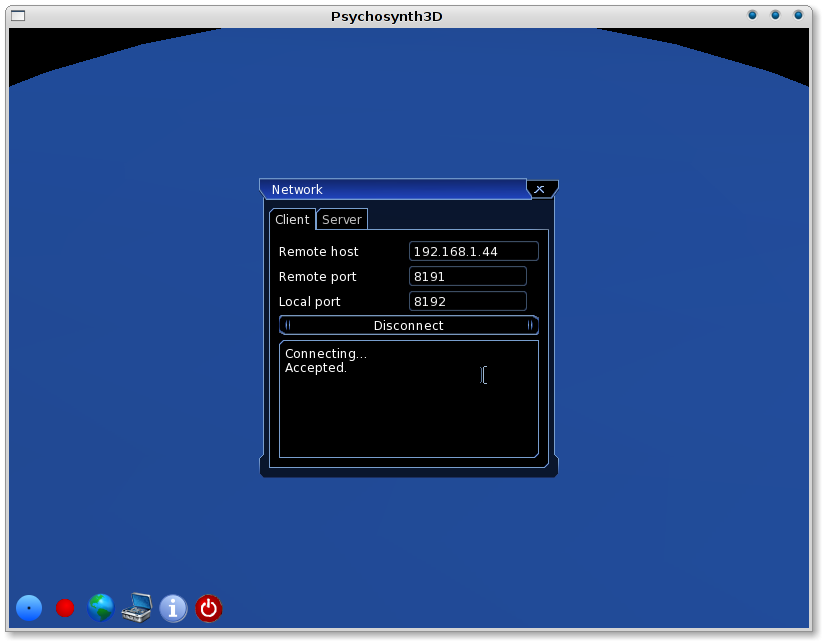
\includegraphics[width=.7\textwidth]{pic/userman-4.png}
  \caption{Successful connection as client in a networked session.}
  \label{fig:userman-4}
\end{figure}

\subsection{Editing options}

The program has various options that we can edit. To do so, we click
on the \emph{toolbox} icon button in the row below. These are the
options that we will find in each category.

\subsubsection{Audio}

Here we can modify the sound generation options. Some of these are:

\begin{description}
\item[Sample rate] The number of audio samples taken per
  second. Higher values give higher quality but need more computer
  power; it is recommended to use the default value. Please note that
  most sound cards only support a specific set of values.

\item[Buffer size] The number of samples that are computed in one
  block. Influences the latency directly, which can be calculated as:
  \begin{equation}
    latency = \frac{buffer\_size}{sample\_rate} seconds
  \end{equation}
  Almost all sound cards require that this number to be a power of
  two. Note that a very low number will cause a greater CPU load and
  potentially cause buffer underruns with annoying clicks at high
  load, while very high values will slow the transfer to the audio
  generation system.

\item[Channels] The number of audio channels. By default stereo sound
  is used.

\item[Output] Choose the output system.
\end{description}

The relative advantages of each setting depend on the platform used
and the use it will give Psychosynth. Normally, depending on the
output system we choose there will be some options available to the
chosen output device.

\subsubsection{Video}

In this section we can change options for the on-screen 3D
environment. Specifically:

\begin{description}
\item[Width and Height] The width and height of the window in
  pixels. fullscreen: Select this for full screen. Note that the apply
  button does not work on systems using GLX due to problems in the
  Ogre library version.

\item[FPS] The refresh rate of the screen in samples per
  second. Higher values consume more CPU power and lower values make
  the animation jerky.
\end{description}

\subsubsection{Paths}

Here we configure the paths where the program searches for data. For
now we can only change where samples are being sought, eg audio files
that we can find in the samples section of the objects selector.

Once we have finished altering the list of search paths click
\emph{refresh} to update the list of samples in the objects
selector. Note that Psychosynth only uses samples that are in
\type{.wav}, \type{.au}, \type{.aiff}, \type{.ogg} or \type{.flac}
format.

\section{The command line interface}

There is a version of the synthesizer that runs from the command line.

In this version we cannot change the environment directly, but we can
use it as a network server, using the option \type{--server} or as a
client in a network using \type{--client}.

We can also hear all the sounds being generated, it is a real
synthesizer; only the state of the scenario is not displayed and
parameters can only be changed through the network.

For complete information on available command line options use
\type{--help}.

%%% Local Variables: 
%%% mode: latex
%%% TeX-master: "00-main"
%%% End: 
